\documentclass[a4paper,12pt]{scrreprt}
    %% Used for changing geometry of the page
    %% Cover page text cannot overlay cover sketching/style 
    %% https://ctan.org/pkg/geometry?lang=en
\usepackage{geometry}
    %% Changes language of some packages protocols
    %% e.g., when captioning images: Figure 1. -> Figura 1.
    %% https://ctan.org/pkg/babel?lang=en
\usepackage[portuguese]{babel}
    %% Used for special fonts
    %% Cannot be compiled with pdflatex
    %% https://ctan.org/pkg/fontspec?lang=en
\usepackage{fontspec}
    %% Arial FONT
    \setmainfont{Arial}

    %% More colors and color options
    %% https://ctan.org/pkg/xcolor?lang=en
    %% https://ctan.org/pkg/colortbl?lang=en
\usepackage{xcolor,colortbl}
    %% More tabular options, like dashed/dotted lines
    %% https://ctan.org/pkg/arydshln?lang=en
\usepackage{arydshln}
    %% List of acronyms
    %% https://ctan.org/pkg/nomencl?lang=en
\usepackage[intoc]{nomencl}
    %% Must be called to init nomencl environment  
    \makenomenclature
    %% More images options/settings
    %% https://ctan.org/pkg/graphicx?lang=en
\usepackage{graphics}
    %% Defining subdirectories to image path enviornment
    %% \graphicspath{{sub1}{sub2}...{subN}}
    \graphicspath{{images}}
    
    %% used to handle cross-referencing commands in LaTeX to produce hypertext links in the document
    %% https://ctan.org/pkg/hyperref?lang=en
\usepackage{hyperref}
    %% math environments
    %% https://ctan.org/pkg/amsmath?lang=en

    %% settings
    \hypersetup{
        colorlinks,
        citecolor=black,
        filecolor=black,
        linkcolor=black,
        urlcolor=black
    }
\usepackage{multirow}
\usepackage[table,xcdraw]{}
%\usepackage{amsmath}
    %% Defining backgrouns, used to make the cover
    %% https://ctan.org/pkg/background?lang=en
\usepackage[some]{background}
    %% Used to make drawings or complex graphics
    %% http://pgf.sourceforge.net/pgf_CVS.pdf
\usepackage{tikz}
    %% Tikz library to point operations ((x1,y1) + (x2,y2))
    \usetikzlibrary{calc}

%% Defining sfdefault font and default font for document
\renewcommand{\familydefault}{\sfdefault}


%% Costume made cover 
%% From there you can use \makecover command to build the cover
%% Blue cover color
\definecolor{titlepagecolor}{RGB}{54,95,145}

%==========================================================================
% COLORED BAR ON THE LEFT SIDE
%==========================================================================

\backgroundsetup{
    scale=1, 
    angle=0, 
    opacity=1,
    contents={
        \begin{tikzpicture}[remember picture,overlay]
            \path [fill=titlepagecolor] 
                (current page.north west) -- ($(current page.north west) + (5,0)$)
                -- ($(current page.south west) + (5,0)$)-- (current page.south west); 
            \node[color=white] at ($(current page.south west) + (3,4)$) {\bfseries {\fontsize{120}{60} \textsf{LI}}};
            \node[color=titlepagecolor] at ($(current page.south west) + (5.8,4)$) {\bfseries {\fontsize{120}{60} \textsf{4}}};
        \end{tikzpicture}
    }
}

%==========================================================================
% TITLE PAGE INFO
%==========================================================================

%% Changes values in this field to show information in the cover and back cover about your team/project


%% TITLE
\title{BonAppetit}

%% AUTHORS
\author{
    Benjamim Miranda Costa ($a87985$)\newline
  \quad
    Maria Sofia Rocha Gomes ($a93314$)\newline
  \quad
    Marisa Ferreira Soares ($a92926$)\newline
  \quad
    Miguel Rodrigues Santa Cruz ($a93194$)
}

%% Date

\date{\today}

%% Course
\newcommand{\Course}{Licenciatura em Engenharia Informática}

%% Department
\newcommand{\Department}{Escola de Engenharia}

%% UniName
\newcommand{\UniName}{Universidade do Minho}

%% UniPic
\newcommand{\UniPic}{
\includegraphics[scale=0.09]{images/uminho.png}}

%% University 
\newcommand{\University}{
    \begin{flushleft}
        \UniPic
    \end{flushleft}
    \textcolor{gray}{\small\textbf{\textsf{\UniName}}}\par
    \textcolor{gray!80!white}{\small{\textsf{\Department}}}\par
    \textcolor{gray!70!white}{\small{\textsf{\Course}}}
}

%% UC
\newcommand{\UC}{
    \begin{flushleft}
        \par\textcolor{titlepagecolor}{  \LARGE\textbf{\textsf{Unidade Curricular de \\ Laboratórios de Informática IV}}}
    \end{flushleft}
}

%% School Year
\newcommand{\SchoolYear}{
    \small{\textsf{Ano Letivo de 2021/2022}}}


%% Define new command to show title, author and date
\makeatletter
\let\Title\@title
\let\Author\@author
\let\Date\@date
\makeatother

%==========================================================================
% CLASSIFICATION SECTION 
%==========================================================================

%% School Year
\newcommand{\ReceptionDate}{}
%% Responsible
\newcommand{\Responsible}{}
%% Evaluation
\newcommand{\Evaluation}{}
%% Observations
\newcommand{\Observations}{}





%% MAKETEMPLATE
\newcommand{\makecover}{

%==========================================================================
% BEGIN COVER PAGE 
%==========================================================================

%% Removes page number on footer
\thispagestyle{empty}

%% No indentation 
\setlength{\parindent}{0em}

%% Put Background defined on \backgroundsetup, in this page
\BgThispage

%% Changing geometry to prevent overlay with text
%% At the end of back cover, geometry is default with \restoregeometry
\newgeometry{top=5cm,left=6cm,right=6cm,bottom=2cm}

%% builds university info defined previously
\University
\vspace{1cm}
%% builds curricular unity info defined previously
\UC
%% builds school year info defined previously
\SchoolYear

\vspace*{5cm}
%% bigger space (i think its the default one) between paragraphs 
\setlength{\parskip}{1em}

%% builds title info defined previously
\par\textbf{\textsf{\huge\Title}}
\vspace{1cm}
%% builds author(s) info defined previously
\par\Author

\vspace{0.5cm}

%% builds date info defined previously
\par\Date
\restoregeometry
\pagebreak

%==========================================================================
% END COVER PAGE 
%==========================================================================

%==========================================================================
% BEGIN BACK COVER PAGE 
%==========================================================================

%% Removes page number on footer
\thispagestyle{empty}

% Changing look of lines in tabular environment 
% Dashed -> dotted 
%% length of dashes
\setlength\dashlinedash{0.3pt}
%% space between dashes
\setlength\dashlinegap{1.5pt}
%% width of dashes
\setlength\arrayrulewidth{1.1pt}


%% This values can be changed in the preamble
\begin{flushright}
\begin{tabular}{ :p{4cm}:p{4cm}: } 
\hdashline
Data de Receção & \ReceptionDate \\ [2ex]
\hdashline
Responsável & \Responsible \\ [2ex]
\hdashline
Avalição & \Evaluation \\ [2ex]
\hdashline
Observações & \Observations \\ [7ex]
\hdashline
\end{tabular}
\end{flushright}


\vspace{10cm}
\begin{flushleft}

%% builds title info defined previously
\par\textbf{\textsf{\huge\Title}}
\vspace{1cm}
%% builds author info defined previously
\par\Author

\vspace{0.5cm}

%% builds date info defined previously
\par\Date
\end{flushleft}

\pagebreak
%==========================================================================
% END BACK COVER PAGE 
%==========================================================================
}


%==========================================================================
% DOCUMENT
%==========================================================================

\begin{document}

\pagenumbering{gobble}

% builds the cover
\makecover

%% smaller footer and header size
\newgeometry{top=3cm,left=3cm,right=3cm,bottom=4cm}




%==========================================================================
% BEGIN ABSTRACT PAGE
%==========================================================================



%% Abstract name: \Large font size, flushed left and paragraph skip before abstract content
\renewenvironment{abstract}
 {\par\noindent\textbf{\Large\abstractname}\par\bigskip}
 {}

\begin{flushleft}
\begin{abstract}
    <<O resumo tem como objectivo descrever de forma sucinta o trabalho realizado. Deverá conter uma pequena introdução, seguida por uma breve descrição do trabalho realizado e terminando com uma indicação sumária do seu estado final. Não deverá exceder as 400 palavras.>> 
    \par \textbf{Área de Aplicação}: Guia de recomendação de locais de consumo de refeições 
    \par \textbf{Palavras-Chave}: Bases de Dados Relacionais, Engenharia de Software, recomendação de restaurantes, aplicação móvel.
\end{abstract}
\end{flushleft}


\pagebreak

%==========================================================================
% END ABSTRACT PAGE 
%==========================================================================

%==========================================================================
% BEGIN INDEXES PAGES
%==========================================================================

%% Changes table of content name
%% Portuguese babel default : "Conteúdo"
%% Personally I prefer "índice"
\renewcommand{\contentsname}{Índice}

\tableofcontents

\pagebreak

\listoffigures

\pagebreak

\listoftables

\pagebreak

%==========================================================================
% END INDEXES PAGES 
%==========================================================================


%==========================================================================
% BEGIN INTRODUCTION
%==========================================================================

%% Starting page numbering here
\pagenumbering{arabic}

    \chapter{Introdução}
        \section{Contextualização}
        \paragraph{}
    Nos últimos anos a economia do mundo ocidental tem sofrido alterações profundas. Os setores primários como a indústria e a agricultura deixaram de ser a principal fonte de riqueza das economias mais desenvolvidas, ocorrendo uma migração para os setores dos serviços e do turismo\cite{ine}. Em Portugal, assim como na União Europeia, o turismo e em particular a área da restauração passou a representar uma fonte de receita fundamental constituindo mais de 5\% do produto interno bruto do bloco europeu segundo o \textit{Eurostat}\cite{eurostat}.
        \paragraph{}
	Apesar de se ter verificado uma diminuição no setor no ano de 2020 devido à pandemia da COVID-19, a restauração nível mundial é ainda um mercado em expansão impulsionado pela revolução digital que passou a permitir mais informação acerca dos estabelecimentos e a divulgação muito mais alargada a nível geográfico.
	\paragraph{}
    Os restaurantes são locais importantes a considerar quando se viaja, contribuindo de forma muito significativa para a experiência no geral. Devido a esta importância é necessário escolher bem o local onde se fazem as refeições, sendo para isso essencial ter informação acerca do restaurante que se pretende frequentar, informações como classificações e críticas de outros utilizadores.
	\paragraph{}
	Numa tentativa explorar este mercado e com o objetivo de ajudar os viajantes surge a necessidade de poder recomendar restaurantes que se adaptem às suas necessidades com a vantagem adicional de promover o comércio local. É com base no anterior referido que se desenvolverá o nosso trabalho: recomendar restaurantes aos utilizadores com base nas suas preferências.
\pagebreak
\section{Motivação e Objectivos}
\paragraph{}
            A gastronomia é provavelmente uma das partes mais importantes e interessantes de viajar, no entanto esta aplicação não se irá basear em restaurantes de comida tradicional e pratos típicos, mas sim todo o tipo de restaurantes. O nosso objetivo é fornecer ao utilizador todo o tipo de opções à sua volta.
            \paragraph{}
            Sendo assim, o principal objetivo no desenvolvimento deste software será promover a restauração e, consequentemente, o turismo e dar a conhecer os diferentes restaurantes de um dado local, permitindo, assim, ao utilizador procurar os estabelecimentos próximos deste e decidir um local para usufruir de uma refeição ao ler experiências de outros utilizadores e, posteriormente, também avaliar e escrever comentários sobre o local.
            Pretendemos o desenvolvimento de uma plataforma de fácil acesso a toda a gente e de utilização simples.
            \paragraph{}
            Outro motivo importante que nos levou a escolher foi o facto da área da restauração ter sido das mais afetadas durante a pandemia do COVID-19, em Portugal. Assim, achámos por bem o desenvolvimento de uma aplicação que o impulsiona o crescimento dessa área.
            \paragraph{}

\section{Justificação e utilidade do sistema}
    \paragraph{}
   Num mundo onde cada vez é mais fácil viajar e conhecer novos locais, muito devido aos avanços tecnológicos, as pessoas não têm paciência ou tempo para estudar antecipadamente os locais do seu destino onde podem fazer uma refeição segundo as suas preferências. Saber as caraterísticas do estabelecimento, se é por exemplo \textit{vegan} ou algo do tipo mais tradicional, é fundamental para efetuar uma escolha informada. Como medida para simplificar este inconveniente surge a \textit{BonAppetit}: uma aplicação móvel, que oferece uma lista de locais onde é possível fazer uma refeição mais próximo do local onde nos encontramos e segundo os nossos gostos pessoais.
   \paragraph{}
    De acordo com as estatísticas realizadas sobre o ano de 2019, em Portugal, existiam cerca de 47062 estabelecimentos de restauração e similares que no total geraram um volume de negocio de 13 994 milhões de euros\cite{ir}.
    
\begin{figure}[htp]
    \centering
    \frame{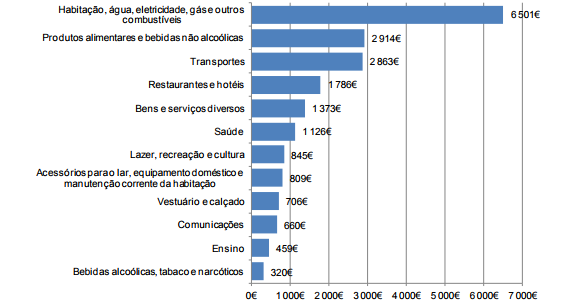
\includegraphics[width=13cm]{images/despesasrestaurantes.png}}
    \caption{Despesa total anual média por agregado e divisões da COICOP, Portugal 2016}
    \label{fig:despesasrestaurantes}
\end{figure}

\paragraph{}
Considerando que os gastos em restauração é a quarta principal despesa anual das famílias podemos concluir que se apenas $0.1\%$ da população utilizasse a nossa aplicação poderíamos gerar uma volume de negócios significativo. Nesse sentido esta aplicação dirige-se a entidades que beneficiem diretamente do aumento do consumo e do turismo nacional, como por exemplo, o governo português ou uma associação de proprietários de estabelecimentos de restauração.
\section{Estabelecimento da identidade do projeto}
\paragraph{}

\graphicspath{ {./images/} }
\begin{center}
\begin{tabular}{ | m{15em} | m{6cm}| } 
  \hline
  Nome  & \textit{BonAppetit} \\ 
  \hline
  Slogan   & "Slogan do projeto" \\ 
  \hline
  Equipa de desenvolvimento & "Equipa de desenvolvimento"  \\ \hline
  
  Características & \bullet  primeiro ponto\newline \bullet  segundo ponto\newline \bullet  terceiroponto \\ \hline
  
  Logótipo  & 
\includegraphics[scale=0.5]{images/icon.png} \\ \hline
  

\end{tabular}
\end{center}

\section{Identificação dos recursos necessários}
    \paragraph{}
    No processo de planeamento de uma aplicação é necessário ter em consideração os recursos que serão utilizados. Um banco de dados  que é povoado pelas informações de cada estabelecimento de restauração é o recurso mais fundamental e para isso teremos que utilizar os seus próprios sites… para criar e gerir esta base de dados.
    \paragraph{}
    Será necessário um dispositivo móvel para testes, um servidor para guardar a base de dados e realizar os diversos serviços que a aplicação poderá oferecer.
    Por outro lado, é necessário 5 pessoas com domínios dos conceitos inerentes à restauração e que saibam também de desenvolvimento de software
\pagebreak
\section{Maqueta do sistema}
\begin{figure}[htp]
    \centering
    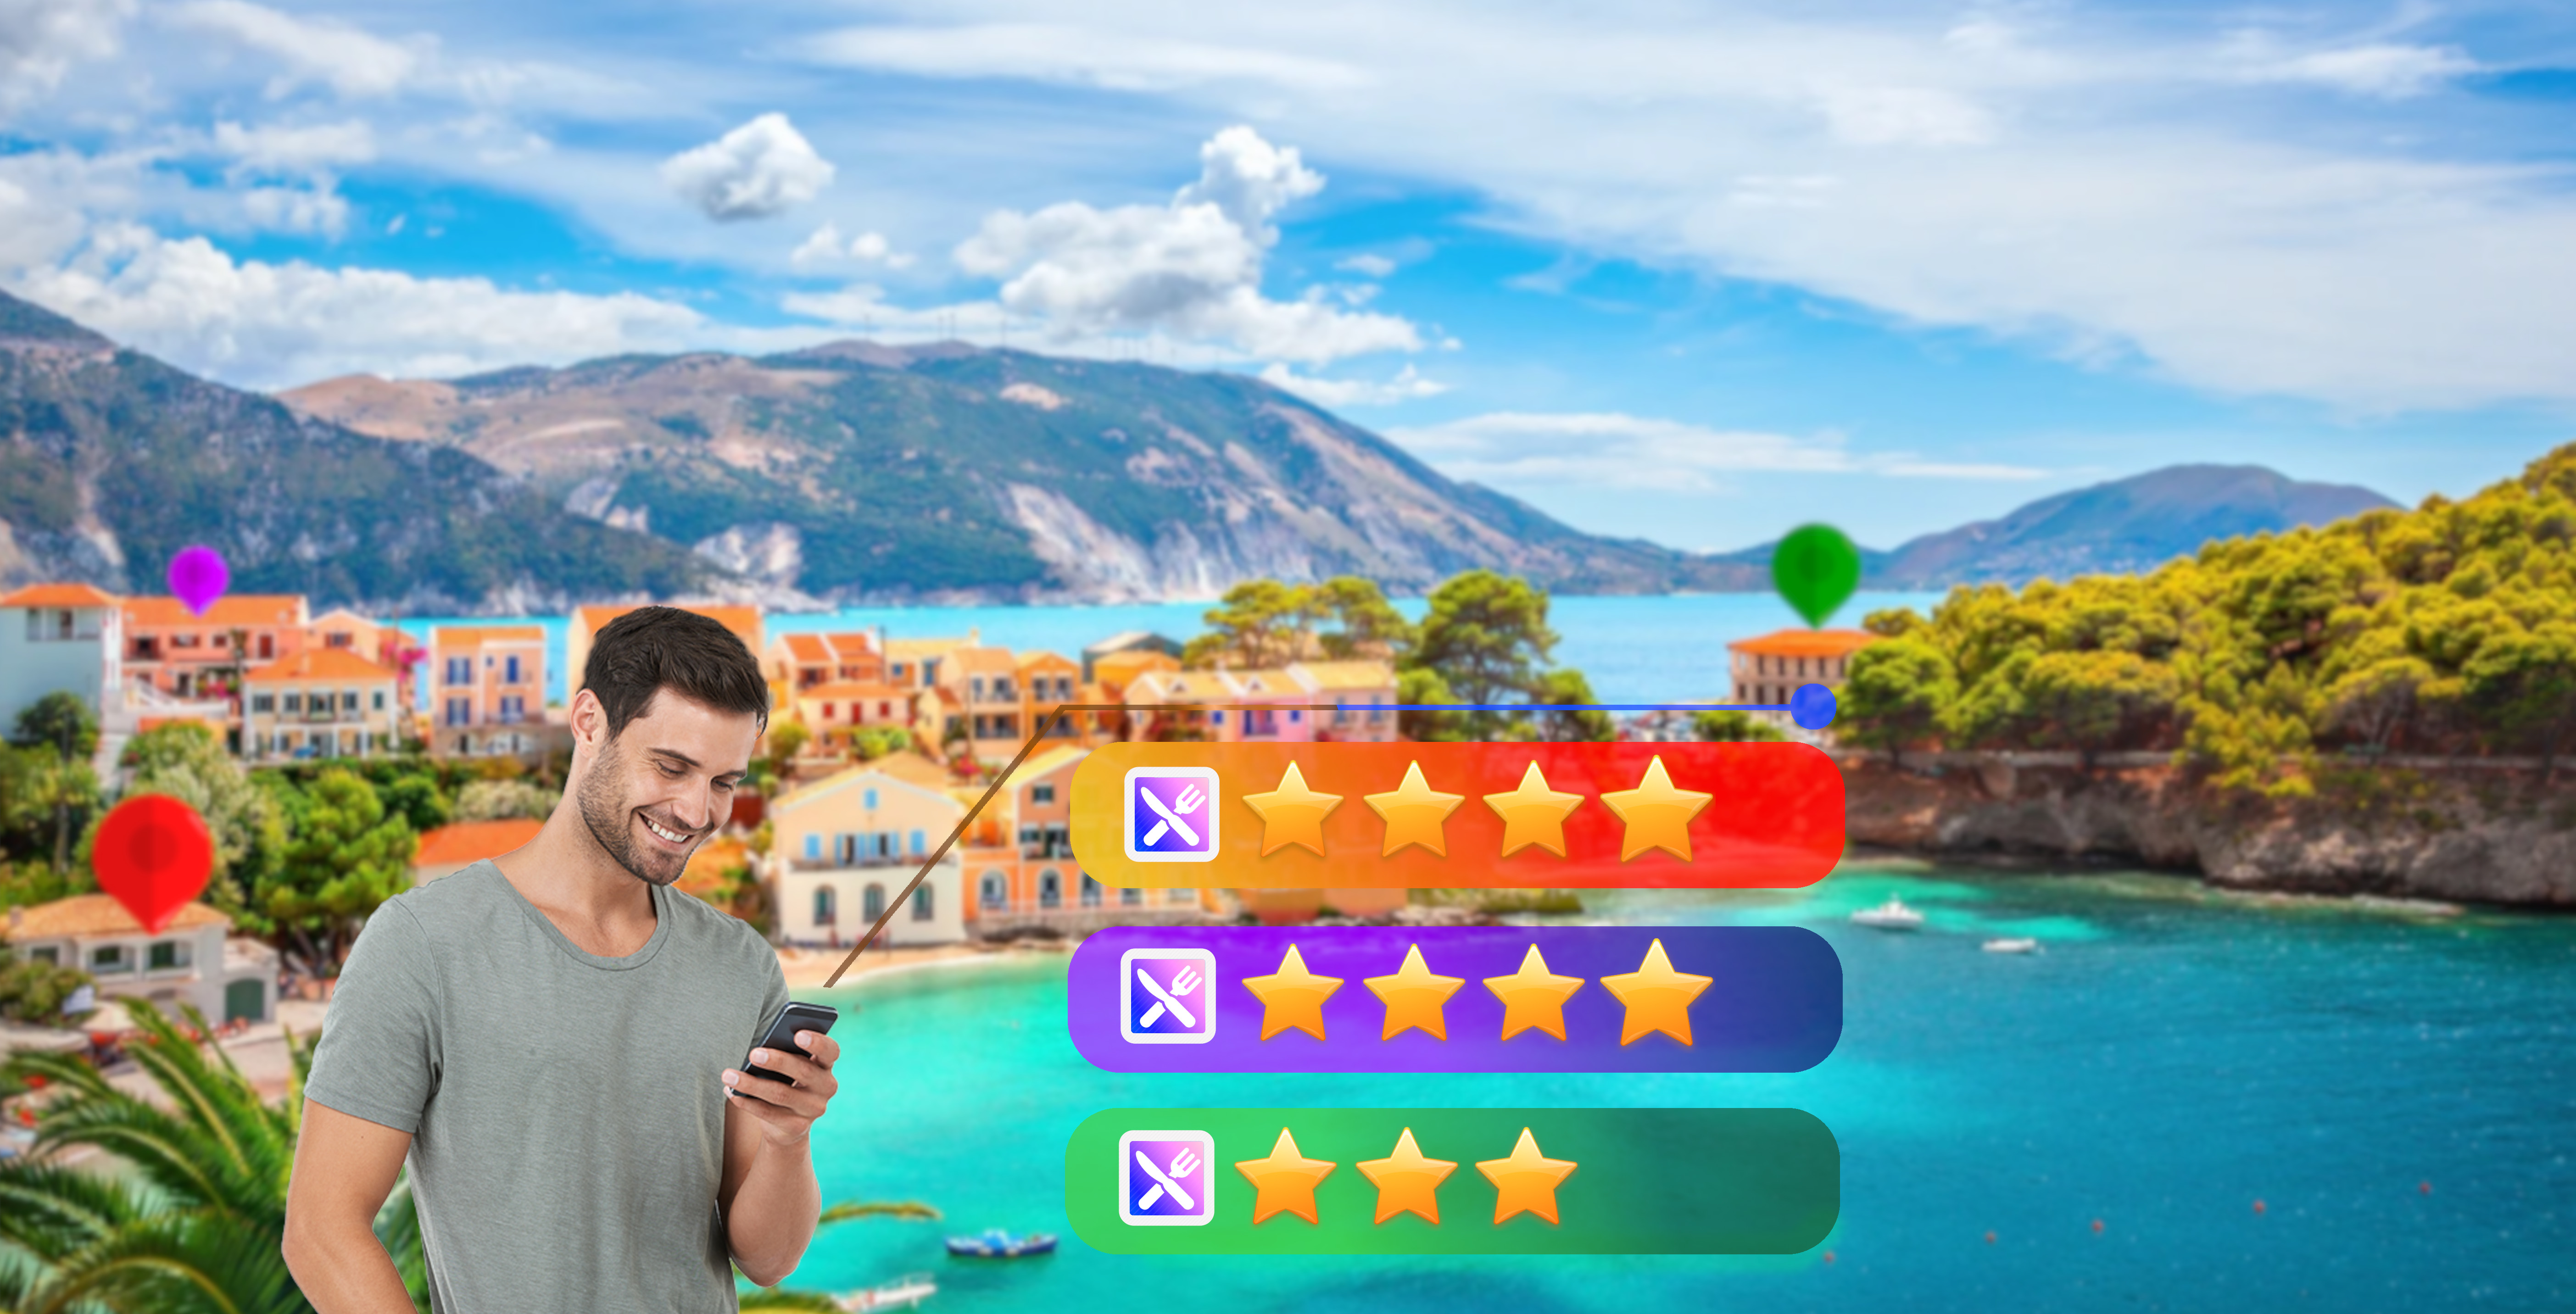
\includegraphics[width=13cm]{images/maqueta.jpg}
    \caption{Maqueta do sistema}
    \label{fig:maquete}
\end{figure}
\paragraph{}
Caso típico de uso da aplicação: utilizador abre a aplicação e vê uma lista de restaurantes próximos e a sua avaliação média ordenados e filtrados com base nas preferências do utilizador.
\section{Medidas de sucesso}
\section{Plano de desenvolvimento}
DIAGRAMA DE GANTT
%==========================================================================
% END INTRODUCTION
%==========================================================================

\chapter{Levantamento e Análise de Requisitos}
        %<< Levantamento e redação dos requisitos do sistema a desenvolver, identificando de forma concreta e
%detalhada as funcionalidades (e restrições) que o sistema deverá ter de forma a satisfazer as necessidades
%apresentadas pelos seus promotores (stakeholders) e utilizadores. O processo de levantamento e de análise
%de requisitos constitui uma das partes mais importantes (senão a mais importante) de um projeto de
%engenharia de software. >>>>>

\section{Apresentação da estratégia e método}
            
\section{Descrição geral dos requisitos (funcionais e não funcionais) levantados}
    \paragraph{}
            Com a utilização desta aplicação, os utilizadores deverão ser capazes de ver uma listagem de restaurantes perto de si, sendo essa a principal funcionalidade. Consequentemente, quando selecionado um local, será possível verificar a avaliação dos restantes utilizadores, bem como os comentários atribuídos. Sendo assim, cada utilizador pode avaliar um restaurante e escrever uma \textit{review}.
            \newline Uma vez marcadas categorias, os restaurantes apresentados serão filtrados por estas, apenas mostrando o que interessa ao utilizador. O utilizador poderá também escolher a ordem pela qual a lista é apresentada: pela avaliação (da melhor à pior e vice-versa) ou pela distância (da menor à maior e vice-versa).
            Caso pretendam aceder à página de um restaurante que não está próximo, o utilizador poderá utilizar a barra de pesquisa e procurar pelo nome do estabelecimento.
            \newline  Para que possam usufruir destas funcionalidades, os utilizadores deverão criar uma conta e autenticar-se.
            Depois do utilizador introduzir as suas informações, o seu endereço de correio eletrónico deverá ser confirmado para finalizar o registo do perfil.
            Assim que criada a conta, será apresentada a página para escolher as categorias pelas quais se interessam mais, não sendo este passo obrigatório. Mais tarde poderão alterar os seus dados pessoais e categorias escolhidas anteriormente.
            \newline{} Segue-se uma lista de requisitos funcionais e não funcionais.\newline

            
            \subsection{Requisitos funcionais:}
           
            \textbf{Registar uma conta} \newline
            Descrição: Para poder utilizar a aplicação, o utilizador deverá criar uma conta. Os dados que deverá fornecer à aplicação serão um \textit{e-mail}, nome próprio, palavra chave e opcionalmente uma foto de perfil.\newline
             • RF01: O utilizador tem de criar uma conta para usar a aplicação. \newline
             • RF02: O sistema deverá pedir os dados mencionados acima para registar.\newline
             • RF03: O sistema terá de enviar um  \textit{e-mail} de confirmação. \newline
             • RF04: O utilizador terá de confirmar o seu  \textit{e-mail}.\newline
             • RF04: O sistema deverá verificar se a password contém no mínimo 8 caracteres.\newline
             • RF05: O utilizador deverá ser identificado pelo  \textit{e-mail}.\newline
            
             
            \textbf{Autenticar} \newline
            Descrição: O utilizador deverá autenticar-se para poder aceder ao conteúdo da aplicação. Para isso deverá usar o mesmo  \textit{e-mail} e palavra passe que utilizou no registo de conta. \newline
            • RF06: O utilizador deverá conseguir autenticar-se.\newline
            • RF07: O sistema tem de pedir \textit{e-mail} e password.\newline
            • RF08: O sistema valida as credenciais introduzidas.\newline
            • RF09: O sistema cancela ou autentica o utilizador na conta.\newline
            
            \textbf{Marcar categorias como favoritas} \newline
            Descrição: Esta será uma das principais funcionalidades do programa. O utilizador deverá escolher as categorias que pretende para que os restaurante sejam filtrados e apresentados de acordo com as suas preferências.\newline
            • RF10: Quando criada a conta, o sistema deverá requisitar ao utilizador que escolha certas categorias dentro duma lista pré-criada.\newline
            
            \textbf{Editar dados da conta} \newline
            Descrição: Uma vez registada a conta e autenticado, o utilizador poderá editar dados fornecidos à aplicação, tais como o nome, password, fotografia e as categorias de preferência. \newline
            • RF11: O utilizador poderá alterar a palavra passe, nome, fotografia e categorias  anteriormente escolhidas.\newline
            • RF12: O sistema deverá validar os dados introduzidos.\newline
            • RF13: O sistema deverá salvar os dados alterados.\newline
            
            \textbf{Procurar por um determinado local.}  \newline
            Descrição: Apesar da aplicação mostrar os restaurantes mais próximos, o utilizador poderá pesquisar por um local específico. \newline
            • RF14: O utilizador deverá poder procurar um estabelecimento, pelo seu nome, na barra de pesquisa.\newline
            • RF15: O sistema deverá apresentar a lista de restaurantes filtrada pelo nome.\newline
            
            \textbf{Listagem de restaurantes} \newline
            • RF16: O sistema deverá apresentar uma listagem de restaurantes filtrados pelas categorias, caso o utilizador tenha alguma selecionada. \newline
            • RF17: O utilizador poderá escolher a ordem pela qual é apresentada a listagem (ordenada por distância ou avaliação).\newline
            • RF18: O sistema deverá apresentar a lista na ordem selecionada pelo utilizador
            
            \textbf{Consultar um restaurante}\newline
            Descrição: O utilizador seleciona um lugar, lê a descrição, avaliação e \textit{reviews} de outros utilizadores. \newline
            RF19: O utilizador deverá abrir a página de um restaurante e consultar as determinadas informações sobre o mesmo, como avaliação e reviews.\newline
            RF20: O sistema deverá apresentar as variadas informações àcerca do restaurante.\newline
            RF21: O utilizador poderá avaliar e deixar o seu comentário sobre um estabelecimento. \newline 
            RF22: O utilizador poderá marcar um local como favorito, de modo a guardar no seu perfil. \newline
            
           \textbf{Consultar listagem de restaurantes favoritos} \newline
            RF23: O utilizador poderá consultar os restaurantes guardados anteriormente 
            \newline
            RF24: O sistema deverá mostrar uma página com os restaurantes salvos previamente.\newline
           
           \textbf{Consultar um mapa} \newline
           RF25: Deverá também ser apresentado ao utilizador um mapa.\newline
           RF26: No mapa deverão estar marcados os locais de interesse do utilizador.\newline

            \textbf{Terminar sessão}
            RF27: O utilizador poderá terminar sessão, uma vez autenticado
            RF28: O sistema terá de terminar a sessão do utilizador.

            \subsection{Requisitos não funcionais:} 
            • RNF01: Em relação ao registo da conta, para confirmar o  \textit{e-mail}, o utilizador possui 10 minutos, caso contrário a conta não é registada. \newline
            • RNF02: A aplicação deve estar operacional 24h por dia.\newline
            • RNF03: ...
            
          
\newpage       
\section{Validação dos requisitos estabelecidos}
\paragraph{}
Para realização de uma primeira versão de requisitos funcionais foi efetuada uma reunião que definiu os primeiros requisitos da aplicação a desenvolver. Por discussão foi feito um refinamento dos requisitos em várias etapas até chegarmos á versão atual, por unanimidade de todos os elementos do grupo.
\paragraph{}
Relativamente ao registo de contas (\textbf{RF01} até \textbf{RF05}) foi referido que é fundamental definir em que contexto é utilizado esse registo. Foi decidido que para utilizar a aplicação é necessário possuir conta para assim o utilizador poder ter uma experiência personalizada. 
\paragraph{}
No sentido de acrescentar detalhes ao processo de registo de conta que não se encontram nos requisitos funcionais consideramos pertinentes as as seguintes informações.
Para efeitos de registo o utilizador terá de fornecer um nome que será mostrado na aplicação dentro menu principal, para identificação da conta, e como nome público nas avaliações e reviews que fizer. O nome não tem nenhuma restrição de formato e poderá ter até 50 caracteres.
Será pedido que defina um endereço de correio eletrónico, não superior a 50 caracteres, que irá posteriormente ser confirmado através de um email de confirmação.
Terá de definir também uma palavra passe que deverá conter pelo menos 8 caracteres onde se encontre pelo menos um caracter numérico e uma letra.
Por fim o utilizador terá a opção de adicionar uma fotografia de perfil numa página própria (explorado mais á frente). É um comportamento válido o utilizador não adicionar nenhuma fotografia, sendo lhe atribuída uma fotografia padrão que deve ser igual para todas as contas que não possuam fotografia definida pelo utilizador.
Para impedir sobrecarregamentos do servidor que conterá a base de dados a tamanho das fotografias estará limitado a 10\textit{MiB}.
A escolha da fotografia padrão bem como o eventual formato e resto dos parâmetros das fotografias adicionadas pelos utilizadores ficam a escolha da equipa de desenvolvedores.
\paragraph{}
Referente à autenticação do cliente (\textbf{RF06} até \textbf{RF09}) acresce dizer que o início de sessão só deve ser efetuado a primeira vez, devendo a aplicação manter o utilizador autenticado até que este queira terminar sessão utilizando o botão que se encontra no menu principal "Terminar sessão".
A utilização de um endereço de correio eletrónico que não tenha sido validado não permitirá concluir o processo de autenticação com sucesso. Apenas se consideram ativas as contas que possuem um endereço de correio eletrónico validado. A validação do endereço de correio eletrónico faz-se abrindo o link contido no email enviado para esse mesmo endereço. Após a abertura do link considera-se a conta validada e não é necessário mais nenhuma ação por parte do utilizador.
\paragraph{}
Relativamente aos detalhes dos restaurantes e ao modo de apresentação dos mesmos importa referir as seguintes informações que não ficaram bem explicitas na formulação dos requisitos funcionais.
Os estabelecimentos possuem:
\begin{itemize}
    \item Logótipo cujo tamanho e formatação ficam ao critério da equipa de desenvolvedores
    \item Nome com um máximo de 50 caracteres
    \item Avaliação média medida em estrelas de zero a cinco com uma casa decimal
    \item Distância ao utilizador medida em metros
    \item Morada completa do estabelecimento (Rua, número de porta,código postal e cidade)
    \item Contactos telefónicos e/ou endereço de correio eletrónico

\end{itemize}





        

\chapter{Especificação e Modelação do Software}
        %<<>>> Apresentação, descrição e representação dos vários elementos e serviços a serem implementados no sistema projeto, utilizando-se, se possível, uma exposição orientada ao serviço suportada por representações UML num nível de abstração adequado.<<<
        
\section{Apresentação geral da especificação}
            
\section{Aspetos estruturais}
            Diagrama de classes , diagrama de componentes, etc..
            modelo de dominio???
\section{Aspetos comportamentais}
        
\begin{table}[htp]
    \begin{center}
        \begin{tabular}{ | m{11em} | m{10cm} | }
          \hline
          Use Case & Registar uma conta \\ 
          \hline
          Ator & Utilizador \\ 
          \hline
          Pré-condição & \textit{True}  \\ 
          \hline
          Pós-condição & 
          • A conta fica registada no sistema.\newline
          • O utilizador fica autenticado.\\ 
          \hline
          Fluxo normal & 
          1. O utilizador fornece ao sistema um e-mail, uma password e nome. \newline
          2. O sistema verifica se já existe conta associada ao e-mail fornecido. \newline
          3. O sistema envia e-mail de confirmação para o utilizador. \newline
          4. O utilizador confirma o e-mail. \newline
          5. O sistema regista a conta.\newline
          6. O utilizador é autenticado.\newline
          7. O sistema apresenta ao utilizador a página inicial.\\ 
          \hline
          \cellcolor{red!50}
           Fluxo de exceção 1 [Já existe uma conta associada ao e-mail] (Passo 2) &  
           1. O sistema avisa que o e-mail já foi utilizado.  \newline
           2. O sistema rejeita o registo da conta. \\
          \hline \cellcolor{yellow!65}
           Fluxo Alternativo 1 [O utilizador não confirmou e-mail]: &
           1. O sistema não regista a conta. \\
           \hline
           
  \end{tabular}
 
\end{center} 
\label{Tab: usecase1}
\caption{Use Case 1 - Registar uma conta}
\end{table}

  
  \begin{table}[htp]
      \begin{center}
        \begin{tabular}{ | m{11em} | m{10cm} | } 
          \hline
          Use case & Escolher categorias \\ 
          \hline
          Ator & Utilizador \\ 
          \hline
          Pré-condição & 
          • Estar autenticado na conta  \\
          \hline
          Pós-condição &
          • As categorias são adicionadas ao perfil do utilizador. \\ 
          \hline
          Fluxo normal & 
          1. O sistema mostra as categorias existentes. \newline
          2. O utilizador escolhe as categorias que pretende. \newline
          3. O sistema guarda as informações introduzidas pelo utilizador. \newline
          4. O sistema apresenta a página inicial.\\ 
          \hline 
  \end{tabular}
\end{center} 
  \label{Tab: usecase2}
\caption{Use Case 2 - Escolher categorias}
\end{table}
  
    \begin{table}[htp]
   \begin{center}
        \begin{tabular}{ | m{11em} | m{10cm} | } 
          \hline
          Use case & Autenticar na conta \\ 
          \hline
          Ator & Utilizador \\ 
          \hline
          Pré-condição & A conta está registada no sistema \\ 
          \hline
          Pós-condição & O utilizador está autenticado. \\ 
          \hline
          Fluxo normal & 
          1. O sistema requere introdução de credenciais.\newline 
          2. Utilizador introduz os dados pedidos.\newline
          3. O sistema verifica que os dados estão corretos. \newline
          4. O sistema autentica o utilizador.\newline
          5. O sistema apresenta a página inicial.\\
          \hline \cellcolor{red!50}
           Fluxo de exceção 1 [Dados introduzidos pelo utilizador não são válidos] &  
           1. O sistema avisa que as credenciais não são válidas.\newline
           2. O sistema não autentica o utilizador.\\ 
           \hline
  \end{tabular}
\end{center} 
  \label{Tab: usecase3}
\caption{Use Case 3 - Autenticar}
\end{table}
   
   \begin{table}[htp]
      \begin{center}
        \begin{tabular}{ | m{11em} | m{10cm} | } 
          \hline
          Use case & Editar dados da conta \\ 
          \hline
          Ator & Utilizador \\ 
          \hline
          Pré-condição & 
          • Estar autenticado na conta \\
          \hline 
          Pós-condição & • Os dados ficam atualizados. \\ 
          \hline
          Fluxo normal &
          1. O sistema mostra os dados do utilizador. \newline
          2. O utilizador altera dados que estão disponíveis para alteração. \newline
          3. Sistema verifica dados fornecidos. \\
          \hline \cellcolor{red!50}
           Fluxo de exceção 1 [A password é inválida] &  
           1. O sistema informa que a password deverá ter no mínimo 8 carateres. \newline
           2. O sistema não atualiza a informação. \\
           \hline
           \cellcolor{red!50}
           Fluxo de exceção 2 [A password alterada é igual] &  
           1. O sistema informa que a password introduzida é a mesma já guardada. \newline
           2. O sistema não atualiza a informação. \\
           \hline
           \cellcolor{red!50}
           Fluxo de exceção 3 [O utilizador cancela a atualização] &  
           1. O sistema cancela a atualização \\ 
           \hline
  \end{tabular}
\end{center}
\label{Tab: usecase4}
\caption{Use Case 4 - Editar dados da conta}
\end{table}

   \begin{table}[htp]
      \begin{center}
        \begin{tabular}{ | m{10em} | m{11cm} | } 
          \hline
          Use case & Editar categorias \\ 
          \hline
          Ator & Utilizador \\ 
          \hline
          Pré-condição & 
          • Estar autenticado na conta  \\
          \hline
          Pós-condição &
          • As categorias são adicionadas ao perfil do utilizador. \\ 
          \hline
          Fluxo normal & 
          1. O sistema mostra as categorias existentes. \newline
          2. O utilizador escolhe as categorias que pretende. \newline
          3. O sistema guarda as informações introduzidas pelo utilizador.\newline
          4. O sistema apresenta a página de edição de dados.\\ 
          \hline 
            \cellcolor{yellow!65}
           Fluxo Alternativo [O utilizador cancela a atualização] &  
           1. O sistema cancela a atualização \\ 
           \hline
  \end{tabular}
\end{center} 
       \label{Tab: usecase5}
\caption{Use Case 5 - Editar categorias}
\end{table}
       
          \begin{table}[htp]
        \begin{center}
        \begin{tabular}{ | m{10em} | m{11cm} | } 
          \hline
          Use case & Ver listagem de restaurantes \\ 
          \hline
          Ator & Utilizador \\ 
          \hline
          Pré-condição & 
          • Estar autenticado na conta  \\
          \hline
          Pós-condição &  \\ 
          \hline
          Fluxo normal & 
          • O sistema apresenta a listagem de restaurantes. \\ 
          \hline 
  \end{tabular}
\end{center} 
\label{Tab: usecase6}
\caption{Use Case 6 - Ver listagem de restaurantes}
\end{table}

\begin{table}[htp]
         \begin{center}
        \begin{tabular}{ | m{10em} | m{11cm} | } 
          \hline
          Use case & Escolher ordem da apresentação da listagem \\ 
          \hline
          Ator & Utilizador \\ 
          \hline
          Pré-condição & 
          • Estar autenticado na conta  \\
          \hline
          Pós-condição &
          • A listagem está ordenada da maneira selecionada \\ 
          \hline
          Fluxo normal & 
          1. O utilizador escolhe que pretende alterar a ordem da lista \newline
          2. O sistema mostra as opções disponíveis. \newline
          3. O utilizador escolhe a pretendida.\newline
          4. O sistema apresenta a lista ordenada da maneira que o utilizador escolheu.\\ 
          \hline 
            \cellcolor{yellow!65}
           Fluxo Alternativo [O utilizador cancela a alteração] &  
           1. O sistema cancela a alteração \\ 
           \hline
  \end{tabular}
\end{center} 
\label{Tab: usecase7}
\caption{Use Case 7 - Alterar a ordem de apresentação da lista}
\end{table}     
        
\chapter{Conceção do Sistema de Dados}
        <<>>> Descrição e caracterização geral do sistema responsável pelo armazenamento da informação requerida pelo sistema que idealizaram e especificaram.
        \section{Apresentação geral da estrutura (esquema) do sistema de dados}
            
        \section{Descrição detalhada dos vários elementos de dados e seus relacionamentos}
        


\chapter{Esboço dos Interfaces do Sistema} 
\section{Estrutura geral das interfaces do sistema}
\begin{figure}[htp]
    \centering
    \frame{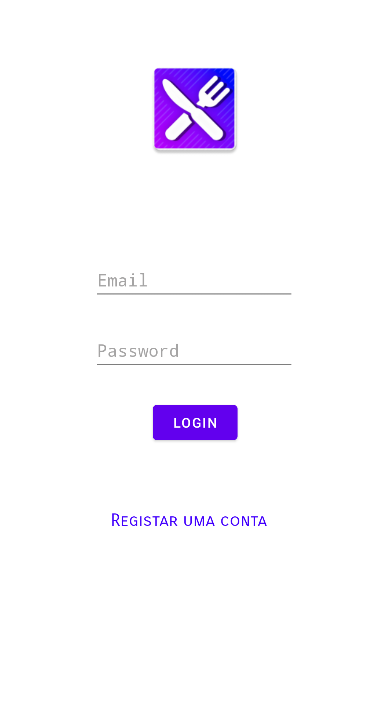
\includegraphics[width=8cm]{images/LOGIN2.PNG}}
    \caption{Página de \textit{login}}
    \label{fig:login}
\end{figure}
\begin{figure}[htp]
    \centering
    \frame{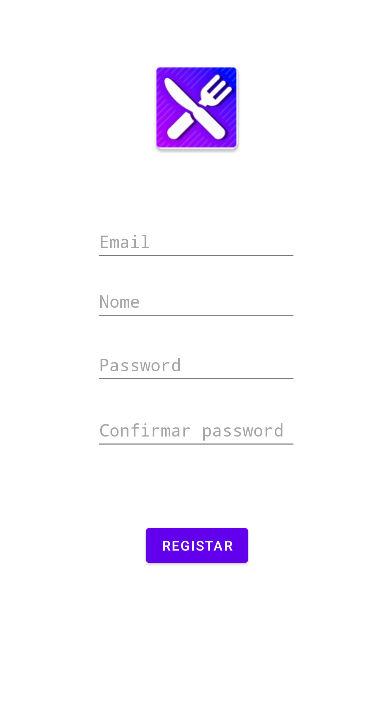
\includegraphics[width=8cm]{images/REGISTAR2.PNG}}
    \caption{Página de registo}
    \label{fig:registo}
\end{figure}
\begin{figure}[htp]
    \centering
    \frame{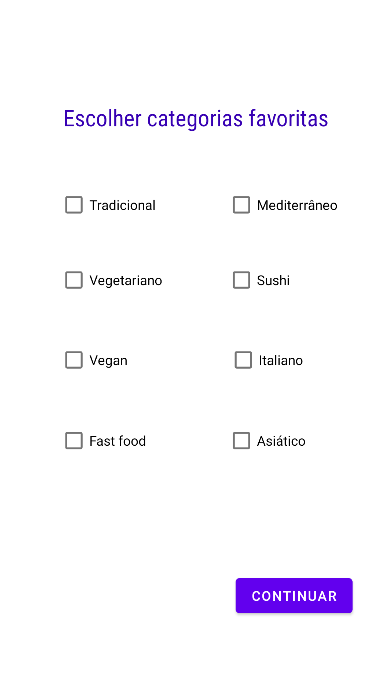
\includegraphics[width=8cm]{images/SELECIONAR CATEGORIAS2.PNG}}
    \caption{Página de seleção de categorias}
    \label{fig:selec}
\end{figure}
\begin{figure}[htp]
    \centering
    \frame{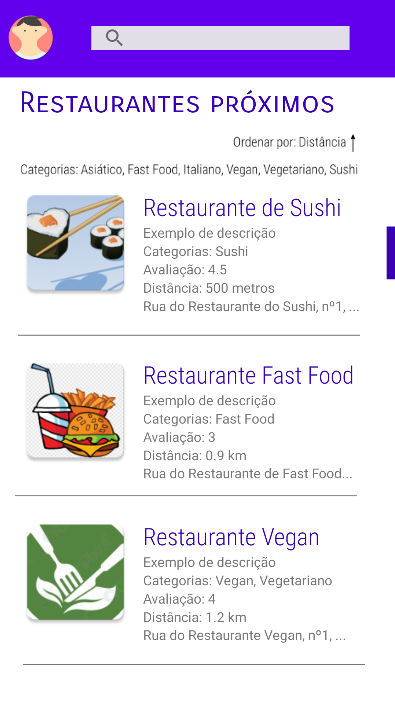
\includegraphics[width=8cm]{images/home.PNG}}
    \caption{Página principal}
    \label{fig:home}
\end{figure}
\begin{figure}[htp]
    \centering
    \frame{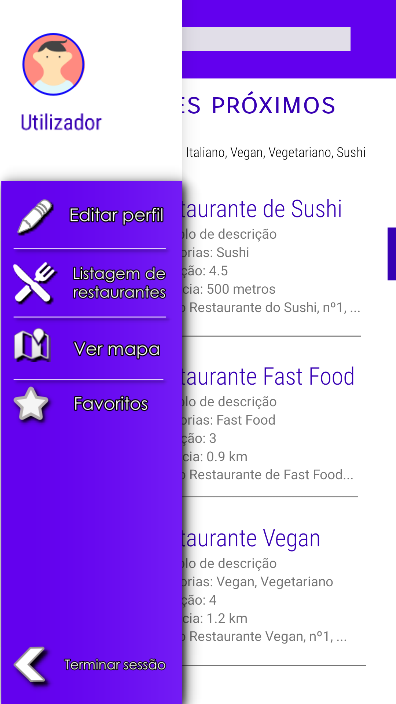
\includegraphics[width=8cm]{images/menu1.PNG}}
    \caption{Menu principal da aplicação}
    \label{fig:menu}
\end{figure}
\begin{figure}[htp]
    \centering
    \frame{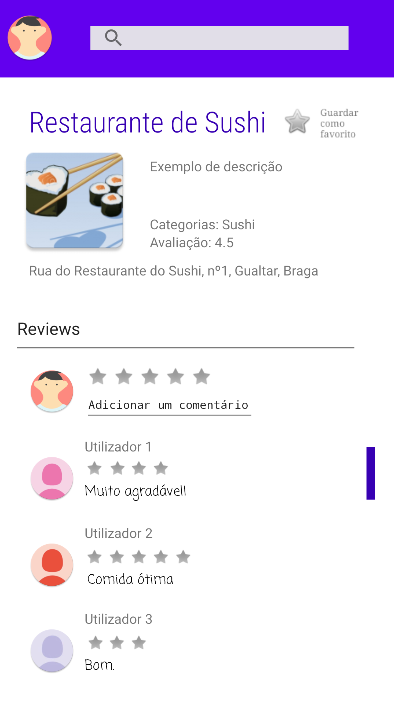
\includegraphics[width=8cm]{images/pagina restaurante1.PNG}}
    \caption{Página de detalhes de restaurante}
    \label{fig:restaurante}
\end{figure}
\begin{figure}[htp]
    \centering
    \frame{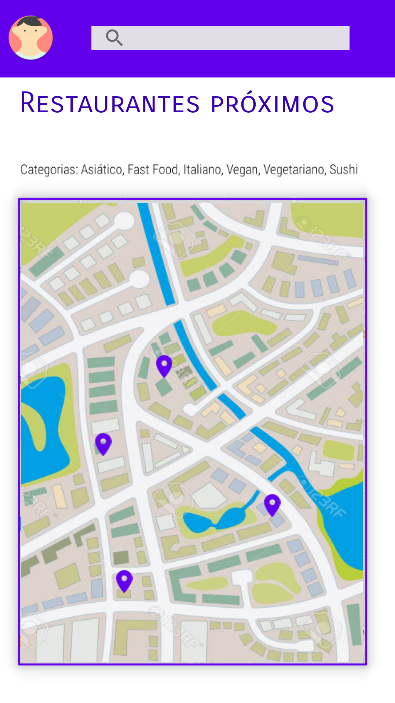
\includegraphics[width=8cm]{images/pagina mapa.PNG}}
    \caption{Mapa de restaurantes próximos}
    \label{fig:mapa}
\end{figure}
\begin{figure}[htp]
    \centering
    \frame{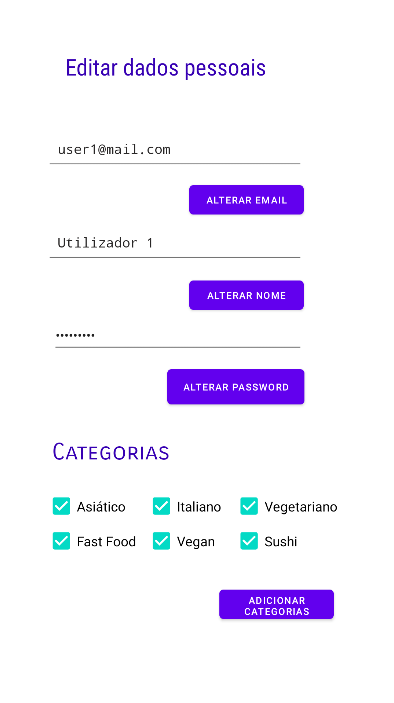
\includegraphics[width=8cm]{images/Editar dados.PNG}}
    \caption{Página de edição de dados pessoais}
    \label{fig:dados}
\end{figure}
        
        
\newpage
\section{Caracterização das interfaces}
\subsection{Páginas de \textit{login} e registo de conta}
\paragraph{}
A página de \textit{login}, representada na figura  \ref{fig:login}, é a primeira interface com que o utilizador vai interagir ao utilizar a aplicação pela primeira vez. Esta página é constituída por duas caixas de texto correspondentes ao endereço de correio eletrónico e á palavra passe do utilizador.
Contém também um botão de ação para efetuar a operação de inicio de sessão e um outro botão para registar uma conta no caso de o utilizador não tiver efetuado o registo previamente.
\paragraph{}
Clicando no botão "Registar uma conta" é mostrado ao utilizador uma nova página, a página de registo de conta representada na figura \ref{fig:registo}.
Nesta página existem quatro campos de introdução de texto. Os dois primeiros pedem ao utilizador para introduzir o seu endereço de correio electrónico e o seu nome sem qualquer restrição de formato.
Os últimos dois campos de introdução de texto referem-se á palavra passe a definir pelo utilizador e a sua respetiva confirmação.
Todo o processo finaliza-se clicando no botão de ação "Registar". 
Durante a introdução do endereço de correio eletrónico e da palavra passe ocorrem verificações sobre a validade dos dados inseridos, como por exemplo, a palavra passe de confirmação não ser igual á palavra passe antes introduzida ou o endereço de correio eletrónico não conter o caracter "@". Sendo detetado algum \textit{input} inválido é mostrada uma indicação visual sob a forma de texto de que algo não se encontra conforme esperado.
\paragraph{}
Estas páginas poderão conter para efeitos de contextualização o ícone da aplicação ou outro efeito decorativo que se considere apropriado.
\subsection{Página de seleção de categorias}
\paragraph{}
A página de seleção de categorias, representada pela figura \ref{fig:selec} é mostrada ao utilizador logo após a conclusão do registo na aplicação. Nela é possível selecionar as categorias favoritas do utilizador para depois ser possível filtrar a lista de restaurantes que é mostrada. Existem nesta página um número de caixas de texto associadas a \textit{checkboxes} igual ao número de categorias definidas pelos desenvolvedores como principais, podendo o utilizador selecionar as categorias que prefere. É ainda um comportamento válido não selecionar nenhuma categoria.
\paragraph{}
O objetivo desta página é fornecer uma lista de todas as categorias existentes de restaurantes ao utilizador para permitir uma primeira personalização das escolhas que mais tarde serão efetivamente mostradas. 
Clicando em "Continuar" o utilizador será levado para a página principal da aplicação.
\paragraph{}
O utilizador terá posteriormente opção de acrescentar mais categorias como favoritas e falo-á sempre através das configurações da aplicação que levaram a esta página.
Assim sendo, esta página é apenas visualizada após a realização do registo e quando se seleciona no menu principal a opção "Editar dados pessoais", não sendo mostrada ao utilizador em nenhuma outra ocasião.
\subsection{Página principal e menu principal}
\paragraph{}
A página principal representada na figura \ref{fig:home} será o ponto de entrada na aplicação depois de o utilizador estar registado e autenticado. Nesta página encontra-se a principal funcionalidade da aplicação: uma lista de restaurantes próximos ordenados por distância ou por avaliações e filtrados com base nas categorias favoritas do utilizador.
Por cada restaurante mostrado são referidas obrigatoriamente os seguintes itens:
\begin{itemize}
  \item Logótipo 
  \item Nome do restaurante
  \item Breve descrição nunca superior a 200 caracteres
  \item Avaliação média do restaurante medida em estrelas de zero a cinco com uma casa decimal.
  \item Distância medida em metros até ao valor de 700, e em quilómetros a partir desse valor
  \item Rua do estabelecimento e número de porta
\end{itemize}
\paragraph{}
No topo da página encontra-se um campo de pesquisa que permite efetuar uma pesquisa global na base de dados de restaurantes. O objetivo deste campo é permitir que se possa avaliar um restaurante visitado após a visita quando já não nos encontremos nas proximidades do mesmo.
\paragraph{}
Clicando na foto do utilizador no canto superior esquerdo ou deslizando do lado esquerdo da página podemos aceder ao menu principal da aplicação. 
\paragraph{}
A figura \ref{fig:menu} representa uma possível implementação do menu principal da aplicação. Este menu permite gerir a conta do utilizador através da opção "Editar perfil", alterar a vista padrão entre lista de restaurantes ou mapa com as opções "Listagem de restaurantes" e "Ver mapa" respectivamente. Permite também consultar a lista de estabelecimentos favoritos com a opção "Favoritos"  e terminar sessão no canto inferior esquerdo com o botão "Terminar sessão", voltando á pagina de \textit{login} já anteriormente referida.
\paragraph{}
A figura \ref{fig:mapa} mostra a visualização dos restaurantes próximos num mapa por contraste com a visualização padrão da lista de restaurantes. Nesta visualização é mostrado um mapa centrado na posição atual do dispositivo com os estabelecimentos marcados por pinos e nome no mapa. Clicando num dos pinos somos levados para a página de informação do restaurante em questão. O mapa implementado deve ser interactivo e suportar \textit{zoom in} e \textit{zoom out} do mesmo.
\subsection{Página de informação de estabelecimento}
\paragraph{}
A página de informação de estabelecimento representada na figura \ref{fig:restaurante} contém a informação do restaurante e é acessada após clicar num restaurante na lista de restaurantes, no mapa ou nos resultados procura global. Nesta página tem de estar presentes os seguintes itens:
\begin{itemize}
  \item Logótipo 
  \item Nome do restaurante
  \item Descrição nunca superior a 500 caracteres
  \item Avaliação média do restaurante medida em estrelas de zero a cinco com uma casa decimal.
  \item Distância medida em metros até ao valor de 700, e em quilómetros a partir desse valor
  \item Morada completa do estabelecimento
  \item Contactos telefónicos ou endereços de correio eletrónico
\end{itemize}
Utilizando o botão "Guardar como favoritos", localizada ao lado do nome do restaurante, é possível adicionar o estabelecimento a uma lista de estabelecimentos favoritos guardados que pode ser consultada a qualquer momento no menu principal.
Nesta página é também possível efetuar avaliações ao estabelecimento usando a caixa de texto "Adicionar um comentário"  e as estrelas que se encontram acima.
É possível consultar as avaliações feitas anteriormente ao estabelecimento por outros utilizadores numa lista ordenada por ordem cronológica.
\subsection{Página de edição de perfil}
\paragraph{}
Na página de edição de perfil é possível mudar os dados pessoais do utilizador como por exemplo o endereço de correio eletrónico, o nome e a palavra passe utilizando para isso as caixas de texto e os respectivos botões. É também possível modificar a foto de perfil do utilizador clicando na sua imagem de perfil, sendo pedido que insira uma nova foto.
Nesta página é também possível editar as categorias favoritas e adicionar novas categorias ás preferências. Clicando no botão "Adicionar categorias" somos levados para a página de seleção de categorias.
\subsection{Interação entre as interfaces}
\begin{figure}[htp]
    \centering
    \frame{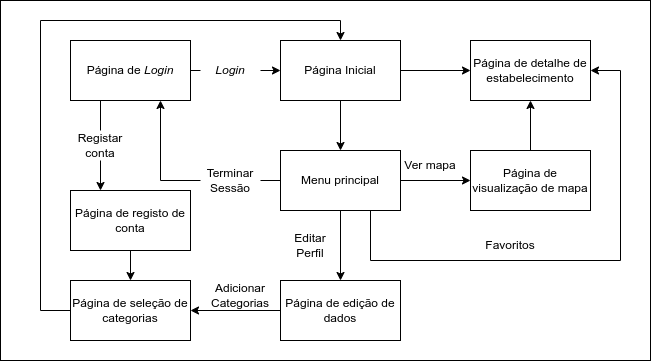
\includegraphics[width=13cm]{images/interacao_interfaces.png}}
    \caption{Relações entre as interfaces da aplicação \textit{BonAppetit}}
    \label{fig:relacoesentreinterfaces}
\end{figure}
\paragraph{}
O diagrama representado na figura \ref{fig:relacoesentreinterfaces} mostra, de uma forma geral, como as interfaces se relacionam entre si e as ações que permitem transitar entre elas.
Existem dois percursos disponíveis para os utilizadores:
\begin{itemize}
    \item Os novos utilizadores começam a interação com a aplicação através da página de \textit{login}. Acedem á pagina de registo, usando o botão "Registar conta", onde vão ser pedidos os dados necessários e já definidos previamente definidos. É em seguida mostrada a página de seleção de categorias favoritas onde podem selecionar ou não as suas preferências e seguem para a página inicial.
    \item Os utilizadores que já possuem conta começam na página de \textit{login} e depois de se autenticarem prosseguem para a página inicial. Os utilizadores só precisam de se autenticar uma vez pois é suposto que da segunda vez que iniciem a aplicação sejam logo levados á página inicial.
\end{itemize}
Partindo da página inicial, que permite aceder ao menu principal deslizando para a esquerda ou clicando na foto de perfil no canto superior esquerdo, é possível aceder a todas as outras interfaces utilizando os botões de ação respectivos.

\chapter{Conclusões e Trabalho Futuro}


\section{Conclusões}
\paragraph{}
Com a realização desta primeira fase tivemos um contacto mais aprofundado com a área da engenharia de software num contexto de especificação de software.
Após a realização desta primeira fase podemos dizer que passamos a compreender a importância de fazer especificação de software, pois esta permite-mos o desenvolvimento do mesmo de uma forma mais sistemática e correta. No entanto temos consciência que só durante na fase de implementação vamos realmente ter completa noção da importância de uma especificação bem realizada.
\paragraph{}
Quanto ao trabalho desenvolvido consideramos que atingimos os objetivos propostos de uma forma geral. 
    
\section{Trabalho futuro}  
-- TO DO -- todos        
        
        
        
        
        
%==========================================================================
% BEGIN SUGESTÕES PARA ESCRITA DO RELATÓRIO
%==========================================================================

%==========================================================================
% END SUGESTÕES PARA ESCRITA DO RELATÓRIO
%==========================================================================

%==========================================================================
% BEGIN CONCLUSÕES DE TRABALHO FUTURO
%==========================================================================



%==========================================================================
% END CONCLUSÕES DE TRABALHO FUTURO
%==========================================================================

%==========================================================================
% BEGIN REFERÊNCIAS
%==========================================================================

%% Changes biblibography name
%% Portuguese babel default : "Bibliografia"
%% Personally I prefer "Referências"
\renewcommand\bibname{Referências}

%% https://www.overleaf.com/learn/latex/bibliography_management_with_bibtex
\begin{thebibliography}{9}

\bibitem{ine}
Instituto Nacional De Estatística,INE. (2018) Tendências macroeconómicas[Online]. Disponível em:
\url{https://www.ine.pt/scripts/european\_economy/bloc-3.html?lang=pt} (Acessado a: 1 de novembro 2021)
\bibitem{eurostat}
Eurostat,E. (2015) Estatísticas sobre o turismo[Online]. Disponível em:
\url{https://ec.europa.eu/eurostat/statistics-explained/index.php?title=Archive:Estat\%C3\%ADsticas\_sobre\_o\_turismo&oldid=220238} (Acessado a: 1 de novembro 2021)
\bibitem{ir}
Banco de Portugal, BPstat. (2021) Análise setorial do alojamento, restauração e similares[Online]. Disponível em:
\url{https://bpstat.bportugal.pt/conteudos/publicacoes/1287} (Acessado a: 1 de novembro 2021)
\bibitem{software_engineering}
Sommerville, I., 2019. Software engineering. 10th ed. Harlow, England: Pearson Education Limited.
\end{thebibliography}


%==========================================================================
% END REFERÊNCIAS
%==========================================================================

%==========================================================================
% BEGIN LISTA DE SIGLAS E ACRÓNIMOS
%==========================================================================

%% Portuguese babel does not translate this environment
\renewcommand{\nomname}{Lista de Siglas e Acrónimos}

%% Text that can be shown before acronyms list
\renewcommand{\nompreamble}{<<Apresentar uma lista com todas as siglas e acrónimos utilizados durante a realização do trabalho. O formato base para esta lista deverá ser da forma como abaixo se apresenta.>>}

%% acronyms
\nomenclature[01]{\textbf{BD}}{Base de Dados}
\nomenclature[02]{\textbf{RF}}{Requisito Funcional}
\nomenclature[03]{\textbf{RNF}}{Requisito Não Funcional}
\nomenclature[04]{DW}{Data Warehouse}
\nomenclature[05]{OLTP}{On-Line Analytical Processing}
\nomenclature[06]{...}{...}

%% Show acronyms
\printnomenclature



%==========================================================================
% END LISTA DE SIGLAS E ACRÓNIMOS
%==========================================================================


%==========================================================================
% BEGIN ANEXOS
%==========================================================================

%% Why \addchap, instead of \chapter? 
%% \addchap has no numbering but appears in table of contents.
\addchap{Anexos}

    <<Os anexos deverão ser utilizados para a inclusão de informação adicional necessária para uma melhor compreensão do relatório o para complementar tópicos, secções ou assuntos abordados. Os anexos criados deverão ser numerados e possuir uma designação. Estes dados permitirão complementar o Índice geral do relatório relativamente à enumeração e apresentação dos diversos anexos.>>
    
    %% section version of \addchap
    \addsec{Anexo 1}


%==========================================================================
% END ANEXOS
%==========================================================================
\end{document}
